\documentclass[11pt]{article}
\usepackage{amsmath,amsthm}
\usepackage{tikz}
\usetikzlibrary{positioning, shapes.misc}
\usepackage{tikz}
\usetikzlibrary{arrows,backgrounds,calc,fit,decorations.pathreplacing,decorations.markings,shapes.geometric}
\tikzset{every fit/.append style=text badly centered}

\begin{document}

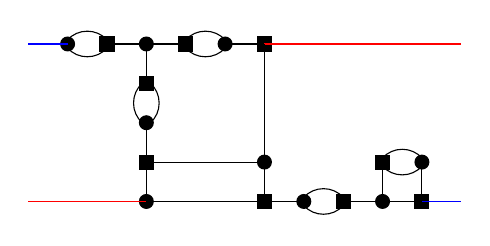
\begin{tikzpicture}[scale=0.5]
  \filldraw (0,0) circle (5pt);
  \draw[black, very thick, fill=black] (-0.15,0.85) rectangle (0.15,1.15);
  \filldraw (0,2) circle (5pt);
  \draw[black, very thick, fill=black] (-0.15,2.85) rectangle (0.15,3.15);
  \filldraw (0,4) circle (5pt);
  \draw[black, very thick, fill=black] (-1.15,3.85) rectangle (-0.85,4.15);
  \filldraw (-2,4) circle (5pt);
  \draw[black, very thick, fill=black] (2.85,-0.15) rectangle (3.15,0.15);
  \draw[black, very thick, fill=black] (0.85,3.85) rectangle (1.15,4.15);
  \filldraw (2,4) circle (5pt);
  \draw[black, very thick, fill=black] (2.85,3.85) rectangle (3.15,4.15);
  \filldraw (3,1) circle (5pt);
  \filldraw (4,0) circle (5pt);
  \draw[black, very thick, fill=black] (4.85,-0.15) rectangle (5.15,0.15);
  \filldraw (6,0) circle (5pt);
  \draw[black, very thick, fill=black] (6.85,-0.15) rectangle (7.15,0.15);
  \draw[black, very thick, fill=black] (5.85, 0.85) rectangle (6.15,1.15);
  \filldraw (7,1) circle (5pt);
  \draw[red] (-3,0) -- (0,0);
  \draw[red] (3,4) -- (8,4);
  \draw[blue] (-2,4) -- (-3,4);
  \draw[blue] (7,0) -- (8,0);
  \draw (0,0) -- (4,0);
  \draw (0,0) -- (0,2);
  \draw (0,3) -- (0,4);
  \draw (-1,4) -- (1,4);
  \draw (2,4) -- (3,4);
  \draw (0,1) -- (3,1);
  \draw (3,0) -- (3,4);
  \draw (5,0) -- (7,0);
  \draw (6,0) -- (6,1);
  \draw (7,0) -- (7,1);
  \draw (-0.1,2) .. controls (-0.4,2.25) and (-0.4,2.75) .. (-0.1,3);
  \draw (0.1,2) .. controls (0.4,2.25) and (0.4,2.75) .. (0.1,3);
  \draw (1,3.9) .. controls (1.25,3.6) and (1.75,3.6) .. (2,3.9);
  \draw (1,4.1) .. controls (1.25,4.4) and (1.75,4.4) .. (2,4.1);
  \draw (4,-0.1) .. controls (4.25,-0.4) and (4.75,-0.4) .. (5,-0.1);
  \draw (4,0.1) .. controls (4.25,0.4) and (4.75,0.4) .. (5,0.1);
  \draw (6,0.9) .. controls (6.25,0.6) and (6.75,0.6) .. (7,0.9);
  \draw (6,1.1) .. controls (6.25,1.4) and (6.75,1.4) .. (7,1.1);
  \draw (-1,4.1) .. controls (-1.25,4.4) and (-1.75,4.4) .. (-2,4.1);
  \draw (-1,3.9) .. controls (-1.25,3.6) and (-1.75,3.6) .. (-2,3.9);
  \end{tikzpicture}

\end{document}